% *********************************************************************
% © 2021–2026 Jeremy Sylvestre
%
% Permission is granted to copy, distribute and/or modify this document
% under the terms of the GNU Free Documentation License, Version 1.3 or
% any later version published by the Free Software Foundation; with no
% Invariant Sections, no Front-Cover Texts, and no Back-Cover Texts. A
% copy of the license is included in the appendix entitled “GNU Free
% Documentation License” that appears in the output document of this
% PreTeXt source code. All trademarks™ are the registered® marks of
% their respective owners.
%
% *********************************************************************

\newcommand*{\xmin}{-2}
\newcommand*{\xmax}{2.75}
\newcommand*{\ymin}{-8}
\newcommand*{\ymax}{17}

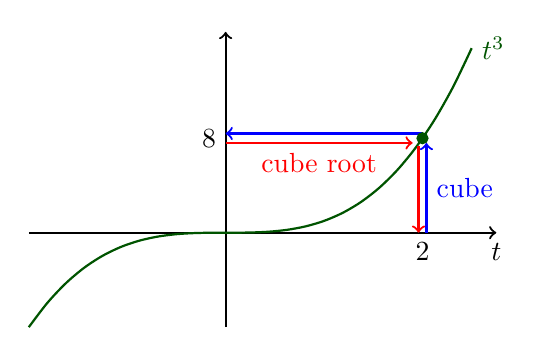
\begin{tikzpicture}
[
	closedpt/.style={circle,draw,fill,inner sep=0pt,minimum size=4pt},
	openpt/.style={circle,draw,inner sep=0pt,minimum size=4pt},
	yscale=0.15,xscale=1.25
]

	% axes
	\draw[->,thick] (\xmin,0) -- (\xmax,0) node[below] {$t$};
	\draw[->,thick] (0,\ymin) -- (0,\ymax);

	\draw[green!33!black,thick,domain=-2:2.5,smooth] plot (\x,{\x * \x * \x}) node[right] {$t^3$};

	\draw[blue,xshift=0.04cm,thick,->] (2,0) -- node[right] {cube} (2,7.6);
	\draw[red,xshift=-0.04cm,thick,->] (2,7.3) -- (2,0);
	\draw[blue,yshift=0.4cm,thick,->] (2,8) -- (0,8);
	\draw[red,yshift=-0.4cm,thick,->] (0,8) -- node[below] {cube root} (1.9,8);

	\node[closedpt,green!33!black] at (2,8) (pt) {};

	\node[below] at (2,0) {$2$};
	\node[left] at (0,8) {$8$};

\end{tikzpicture}
